\documentclass[a4paper]{article}
\usepackage[english]{babel}
\usepackage{amsmath}
\usepackage{graphicx}
\usepackage{placeins}
\usepackage{booktabs}

\title{Building Evacuation}
\author{Maarten de Jonge \\
        Edwin Odijk \\
        Roelof van der Heijden}

\begin{document}

\maketitle

\section{Introduction}
In this report we simulate people escaping from a burning building using the BDI framework in NetLogo. We create an environment with people and fire randomly distributed throughout the building. People randomly walk through the building until they spot fire, at which point they try to run towards the escape and alarm any others they meet along their way. The simulation ends when all people either escaped or died in a fire.

Using this simulation, we aim to find what affects the speed and survival rate of such an evacuation.

Additionally, we describe the NetLogo implementation, explaining the functions of buttons and how they are implemented.

\section{Environment}
\FloatBarrier
The simulation environment is a 33x33 grid, representing an office space (Figure~
\ref{fig:office}). The walls (black tiles) were hand-drawn to craft a somewhat
realistic layout of rooms and hallways. One exit (green tile) is placed
randomly, as well as a variable number of initial fires (red tiles). Care is
taken to ensure the exit is reachable, i.e. it is not inside a wall or on fire.

\begin{figure}[h!]
  \centering
  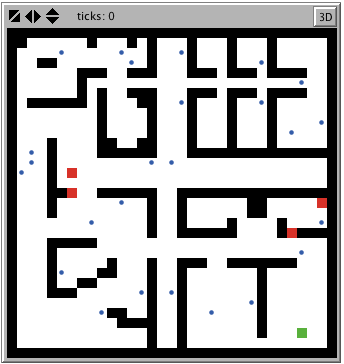
\includegraphics[width=0.5\textwidth]{office.png}
  \label{fig:office}
  \caption{The office layout, with random fires and exit}
\end{figure}

A variable amount of people (ranging from 1 to 25) is spawned, again making sure
not to doom them by spawning them inside walls or fires. At each tick of the
simulation, 

\subsection{Agents}
The agents represent people trying to escape the burning building.
Following the BDI framework, the agents possess the beliefs, desires and
intentions described in Table \ref{tbl:bdi}.
\begin{table}[h!]
  \centering
  \begin{tabular}{lll}
    \toprule
    Beliefs & Desires & Intentions \\
    \midrule
    Locations of walls & Roam around & Move towards exit \\
    Locations of fire & Escape & Alarm other agents of fire \\
    Location of exit & & Roam around \\
    \bottomrule
  \end{tabular}
  \caption{Agents in the BDI framework}
  \label{tbl:bdi}
\end{table}

Additionally, each agent has a variable vision radius for both detecting fire
and detecting people to alarm.

TODO: detail the flow of desires and intentions

\subsection{NetLogo Controls}
To provide more insight in the workings of this simulation, we provide a overview below of the controls implemented in NetLogo, as not all of them may be self-explanatory.

\subsubsection{Draw, Save and Clear walls}
Walls used by the simulation are handdrawn and saved in a separate txt file. Upon running Setup, the file is read to redraw the walls.

To use the function, first ensure that Setup is run at least once. If walls are already present, you can click clear\_walls (thereby removing the txt file) and run Setup again to redraw the environment with an empty sheet. Clicking draw\_walls allows you to start drawing with the environment. When you are finished, click draw\_walls again to stop drawing, then click save\_walls to save the new environment, which will now be redrawn every time Setup is run.

\subsubsection{Throttle Speed}
As the simulation may slow down at times, it may be preferrable to watch the simulation at a constant speed. Turning throttle\_speed on slows all steps to an equal speed of 100 milliseconds. This does mean that the overall speed of the simulation is slowed down, however, so this should be off when swift simulations are desired.

\subsubsection{Fire Spread Rate}
Controls the speed at which fire spreads. At every step, fire may spread to each neighbouring tile with a probability defined by fire\_spread\_rate in promille for each of these tiles.

\subsubsection{Vision}
The properties fire\_vision and person\_vision control the vision in which each agent can observe nearby fire or other agents respectively. This vision is represented by an invisible circle around the agent, with a radius equal to the value defined on the slider.

\FloatBarrier
\section{Experiments}
\begin{itemize}
\item Can we prevent traffic jam behaviour?
\item How much do the following properties affect overall survival rate?
\begin{itemize}
\item Rate at which fire spreads
\item Whether agents have prior knowledge of exit locations
\item The ratio between agents that prioritize saving themselves over saving others
\end{itemize}
\end{itemize}

\section{Results}

\section{Conclusion}

\section{Future Work}
There are various potential improvements to the simulation that haven't been
implemented due to time constraints. Regarding the simulation environment, it
would be interesting to automatically generate an office layout based on some
parameters (e.g. number of exits, wall density, width of corridors, number of
open areas). This would allow for research to be done into the effect of the
layout on, for instance, the survival rate or some measure of traffic congestion.

The agents themselves could be parameterised by some measure of personality; for
example, they could have a probabilistic bias towards warning their colleagues,
or conversely a bias towards saving themselves without regards for the others.
This could even be extended to replicate real-world fire safety procedures where
certain agents (presumably wearing fluorescent yellow jackets) are tasked with
making sure all the other agents are aware of the fire before fleeing themselves.

\end{document}